\documentclass[aps,prb,longbibliography,superscriptaddress,twocolumn]{revtex4-2}
\usepackage{graphicx,caption}
\usepackage{mathtools,amsmath,amssymb}
\usepackage{physics}
\usepackage{here}
\usepackage{multirow}
\usepackage{xcolor}
\usepackage{hyperref}

\def\be#1\ee{\begin{align}#1\end{align}}

%%%%%%%%%%%%%%%%%%%%%%%%%%%%%%%%%%%%%%%%%%%%%%%%%%%%%%%%%%%%%%%%%%%%%%%%%%%%%%

\begin{document}
\title{Inverse Faraday Effect Induced by the Quantum Geometry}

\author{Hiroki Yoshida}
\affiliation{Department of Physics, Institute of Science Tokyo, 2-12-1 Ookayama, Meguro-ku, Tokyo 152-8551, Japan}
\author{Takehito Yokoyama}
\affiliation{Department of Physics, Institute of Science Tokyo, 2-12-1 Ookayama, Meguro-ku, Tokyo 152-8551, Japan}


\date{\today}


\begin{abstract}
    We propose a novel mechanism of the inverse Faraday effect arising from a quantum geometric origin, characterized by the quantum metric dipole. Within a semiclassical framework based on the Boltzmann transport theory, we establish a general formalism describing light-induced magnetization in electronic systems as a second-order nonlinear response to the electric field of light. We show that this effect is activated by a spatially non-uniform electric field component and, in contrast to the conventional inverse Faraday effect, persists even under linearly polarized illumination. Model calculations reveal that the magnitude of the resulting magnetization is comparable to that induced in conventional inverse Faraday effect by circularly polarized light, indicating its experimental realizability. Our results highlight a direct manifestation of the quantum metric dipole in nonlinear optical responses and suggest a viable pathway for its experimental detection.
\end{abstract}

\maketitle

The Faraday effect is one of the most prominent magneto-optical phenomena, characterized by the rotation of the polarization plane of light as it propagates through a magnetized medium~\cite{Faraday_1846}. Its counterpart, the inverse Faraday effect (IFE), refers to the generation of magnetization in a material in response to light. The IFE has been both theoretically predicted~\cite{Pitaevskii_1961,Pershan_1963} and experimentally confirmed~\cite{Zeil_Optically_1965}, and is typically described as a second-order optical response, with the induced magnetization being proportional to the cross product of the electric field and its complex conjugate. As a consequence, the IFE is conventionally associated with circularly polarized light. Both the Faraday and inverse Faraday effects now play central roles in the optical manipulation and probing of magnetization in condensed matter systems.

Nonlinear optical effects--which arise from higher-order responses (second order or above) to the electric and magnetic fields of light--have garnered growing theoretical interest in recent years. This attention is largely driven by their profound connection to quantum geometry. A paradigmatic example is the bulk photovoltaic effect~\cite{kraut.vonbaltz1979a,belinicher.sturman1980,vonbaltz.kraut1981a,aversa.sipe1995a,sipe.shkrebtii2000,fridkin2001}, a second-order response to the electric field, where the nonlinear conductivity can be expressed in terms of geometric quantities such as the Berry curvature~\cite{morimoto.nagaosa2016,morimoto.nagaosa2016b,ma.etal2021,ahn.etal2022}. Other nonlinear transport phenomena, such as the nonlinear Hall effect is known to be related with the Berry curvature dipole~\cite{Fu_2015}. Also, different geometric quantity known as a quantum metric dipole can appear in nonlinear Hall effect~\cite{Gao_positional_2014,Liu_2021,Kamal_2023,Gao_Science_2023}. Nevertheless, the influence of quantum geometry on the inverse Faraday effect remains largely unexplored.

In this letter, we unveil a novel mechanism of light-induced magnetization in electronic systems, mediated by quantum geometric effects. We consider spatially non-uniform light, characterized by an electric field with explicit position dependence. This spatial variation modifies the semiclassical equation of motion for electrons~\cite{Lapa_Hughes_2019}, which in turn alters the second-order current response derived from the Boltzmann transport equation. The resulting current, arising from the spatial inhomogeneity of the electric field, can be interpreted as a magnetization current, allowing us to derive an expression for light-induced magnetization as a second-order response to the electric field. This effect originates from Fermi surface contributions and is therefore relevant only in metallic systems. Remarkably, unlike the conventional inverse Faraday effect, it can be induced even by linearly polarized light. We further demonstrate the magnitude of this effect through a model calculation based on a simple Dirac Hamiltonian.

We start from the semiclassical equation of motion of an electron under non-uniform electric field. Throughout this paper, we ignore the effect of magnetic field of light and concentrate on the electric field. Under such approximation, we can ignore the time-derivative of the vector potential by adopting appropriate gauge and the analysis is almost same as the one for time-independent electric field. Then, our setup is the same as in Ref.~\cite{Lapa_Hughes_2019}. The Hamiltonian of the system is given as
\be
    \hat{H}&=\hat{H}_0+Q\varphi(\hat{\vb{x}}),
\ee
where $\hat{H}_0$ is a static Hamiltonian including a periodic potential, $Q=-e$ is the charge of an electron, and $\phi$ is a scalar potential that gives the electric field $E_{\mu}=-\pdv{\varphi}{x_{\mu}}\ (\mu=x,y,z)$. We expand the position-dependent electric field $\vb{E}(\vb{x})$ around the origin as 
\be
    E_{\mu}(\vb{x})&=e_{\mu}+e_{\mu\nu}x_{\nu},
\ee
where $e_{\mu}=E_{\mu}(\vb{x}=\vb{0})$ and $e_{\mu\nu}=\pdv{E_{\mu}}{x_{\nu}}\eval_{\vb{x}=\vb{0}}$ are the electric field and its gradient at the origin, respectively. Because the electric field is a gradient of the scalar potential, $e_{\mu\nu}=e_{\nu\mu}$. In Ref.~\cite{Lapa_Hughes_2019}, the equation of motion (EOM) of an electron in this setting is derived as
\be
    \dot{x}_{\mu}&=\frac{1}{\hbar}\pdv{\varepsilon}{k_{\mu}}-\Omega_{\mu\nu}\dot{k}_{\nu}-\frac{1}{2\hbar}Qe_{\nu\lambda}\pdv{g_{\nu\lambda}}{k_{\mu}},\label{eq:EOM_x}\\
    \dot{k_{\mu}}&=\frac{1}{\hbar}QE_{\mu}(\vb{x})\label{eq:EOM_k}.
\ee
Here, $\varepsilon$ is the energy of the electron satisfying $\hat{H}_0\ket{\phi(\vb{k})}=\varepsilon(\vb{k})\ket{\phi(\vb{k})}$. The single-band Bloch state can be written as $\ket{\phi(\vb{k})}=e^{i\vb{k}\cdot\vb{x}}\ket{u(\vb{k})}$, $\Omega_{\mu\nu}\coloneqq i\qty(\bra{\pdv{u}{k_{\mu}}}\ket{\pdv{u}{k_{\nu}}}-\qty(\mu\leftrightarrow\nu))$ is the Berry curvature, and
\be
    g_{\mu\nu}\coloneqq \frac{1}{2}\qty(\bra{\pdv{u}{k_{\mu}}}\ket{\pdv{u}{k_{\nu}}}-\bra{\pdv{u}{k_{\mu}}}\ket{u}\bra{u}\ket{\pdv{u}{k_{\nu}}}+\qty(\mu\leftrightarrow\nu))
\ee
is the quantum metric. These two quantities correspond to the imaginary and real parts of the quantum geometric tensor~\cite{Provost_1980}, respectively. In the equations of motion, the first term of Eq.~\eqref{eq:EOM_x} is the conventional term showing the group velocity. Equation~\eqref{eq:EOM_k} and the second term of Eq.~\eqref{eq:EOM_x} include the effect of an applied electric field. The third term of Eq.~\eqref{eq:EOM_x} is unique to the non-uniform electric field.

From the EOMs, we next calculate the electric current density of this system using the Boltzmann formalism. The Boltzmann equation with relaxation time approximation can be written as
\be
    \pdv{f}{t}+\dot{\vb{x}}\cdot\pdv{f}{\vb{x}}+\dot{\vb{k}}\cdot\pdv{f}{\vb{k}}=-\frac{f-f_0}{\tau},
\ee
where $f$ is the distribution function of the system, $f_0$ is the equilibrium Fermi distribution function, and $\tau$ is the relaxation time of an electron. We calculate the change of the distribution function $f-f_0$ up to a first order of $\tau$. In this case, $f$ in the left hand side can be approximated to be $f_0$. Using facts that the state is in equilibrium $\pdv{f_0}{t}=0$ and uniform $\pdv{f_0}{\vb{x}}=\vb{0}$, we get
\be
    f&\approx f_0+\frac{\tau Q}{\hbar}E_{\mu}(\vb{x})\pdv{f_0}{k_{\mu}}.
\ee
This distribution function has the same form as the one under a uniform electric field. Using this distribution function, the electric current density $j_{\mu}\coloneqq Q\int[\mathrm{d}\vb{k}]f\dot{x}_{\mu}$ can be calculated as
\begin{widetext}
    \be
        j_{\mu}&=\frac{Q}{\hbar}\int[\mathrm{d}\vb{k}]f_0\pdv{\varepsilon}{k_{\mu}}+\qty(\frac{\tau Q^2}{\hbar^2}\int[\mathrm{d}\vb{k}]\pdv{f_0}{k_{\nu}}\pdv{\varepsilon}{k_{\mu}}-\frac{Q^2}{\hbar}\int[\mathrm{d}\vb{k}]f_0\Omega_{\mu\nu})E_{\nu}(\vb{x})-\frac{Q^2}{2\hbar}\int[\mathrm{d}\vb{k}]f_0\pdv{g_{\nu\lambda}}{k_{\mu}}e_{\nu\lambda}\nonumber\\
        &\hspace{7cm} -\frac{\tau Q^3}{\hbar^2}\int[\mathrm{d}\vb{k}]\pdv{f_0}{k_{\nu}}\Omega_{\mu\gamma}E_{\nu}E_{\gamma}-\frac{\tau Q^3}{2\hbar^2}\int[\mathrm{d}\vb{k}]\pdv{f_0}{k_{\gamma}}\pdv{g_{\nu\lambda}}{k_{\mu}}E_{\gamma}e_{\nu\lambda}.\label{eq:current_general}
    \ee
\end{widetext}
Here, $\qty[\mathrm{d}\vb{k}] = \frac{\mathrm{d}\vb{k}}{(2\pi)^d}$ with the dimension of the system $d$ and the integration is over the whole Brillouin zone. The first three terms in Eq.~\eqref{eq:current_general} represent conventional currents caused by the application of an electric field. In Ref.~\cite{Lapa_Hughes_2019}, the fourth term is referred as the ``geometric'' current. This geometric current is caused by the gradient of the electric field and quantum metric. Using integration by parts, this current can be calculated as a Fermi surface integration of the quantum metric. The last two terms are the second-order response to the applied electric field. They are represented also as Fermi surface integrations of Berry curvature and the derivative of the quantum metric (metric dipole), respectively and thus, only present in metallic systems.

We next turn our attention to the magnetization. In a system with magnetization $\vb{M}$, the associated magnetization current is defined as
\be
    \vb{j}_{\mathrm{mag}}&\coloneqq\curl{\vb{M}},
\ee
where $\nabla$ is the derivative with respect to the real space coordinates. We focus on a magnetization that is induced as a second-order response to the electric field of light and assume that
\be
    M_{\alpha}(\vb{x})&=a_{\alpha\beta\gamma}E_{\beta}(\vb{x})E_{\gamma}(\vb{x}).\label{eq:M_def}
\ee
Then, the magnetization current caused by this magnetization can be calculated as
\be
    j_{\mathrm{mag},\mu}(\vb{x}) &=-2\varepsilon_{\mu\nu\alpha}a_{\alpha\gamma\lambda}E_{\gamma}(\vb{x})e_{\lambda\nu},
\ee
up to the first order expansion of the electric field with respect to the position. Then, as $e_{\lambda\nu}=e_{\nu\lambda}$, the magnetization current can be written as
\be
    j_{\mathrm{mag},\mu}&=-2\varepsilon_{\mu\nu\alpha}a_{\alpha\gamma\lambda}e_{\gamma}e_{\lambda\nu}.
\ee
In the general expression of the current in Eq.~\eqref{eq:current_general}, the last term has the same form as this current, depending on the zeroth- and first-order derivatives of the electric field. Therefore, the last term of Eq.~\eqref{eq:current_general} can be understood as a magnetization current caused by a magnetization $\vb{M}$ induced by the light, i.e. by IFE. By comparing two expressions, we find
\be
    \varepsilon_{\mu\nu\alpha}a_{\alpha\gamma\lambda}&=\frac{\tau Q^3}{4\hbar^2}\int[\mathrm{d}\vb{k}]\pdv{f_0}{k_{\gamma}}\pdv{g_{\nu\lambda}}{k_{\mu}}.
\ee
Integrating by parts, we get a formula of the coefficient defined in Eq.~\eqref{eq:M_def} for the IFE caused by the non-uniform electric fields as
\be
    a_{\mu\alpha\beta}&=-\frac{\tau Q^3}{\hbar^2}\varepsilon_{\mu\nu\delta}\int[\mathrm{d}\vb{k}]f_0\pdv[2]{g_{\delta\beta}}{k_{\alpha}}{k_{\nu}}\label{eq:coeff_metric}
\ee
This is our main result. This coefficient is proportional to a quadrupole-like quantity of the quantum metric $\int[\mathrm{d}\vb{k}]f_0\partial_{k_{\alpha}}\partial_{k_{\nu}}g_{\delta\beta}$, referred to as the \textit{quantum metric quadrupole}. This quantity has been studied in the context of third-order electric responses~. In our case, only the antisymmetric part of the quantum metric dipole is responsible for the generation of the IFE. Note that even when $\alpha=\beta$, where the illuminated light is linearly polarized, this effect, can be non-zero in general. This is a clear distinction from the conventional IFE, where magnetization can only be induced for circularly polarized light.

We can rewrite the expression~\eqref{eq:coeff_metric} using the Christoffel symbol which highlights the connection between gravity and quantum geometric nature of the effect. From the quantum metric, Christoffel symbol can be defined as
\be
    \Gamma_{\alpha\beta\gamma}&\coloneqq\frac{1}{2}\qty(\partial_{k_{\gamma}}g_{\alpha\beta}+\partial_{k_{\beta}}g_{\alpha\gamma}-\partial_{k_{\alpha}}g_{\beta\gamma}).
\ee
Then, it is easy to see
\be
    \partial_{k_{\gamma}}g_{\alpha\beta}&=\Gamma_{\alpha\beta\gamma}+\Gamma_{\beta\alpha\gamma},
\ee
meaning that the quantum metric dipole~\cite{Gao_positional_2014,Liu_2021,Kamal_2023,Gao_Science_2023} $\partial_{k_{\gamma}} g_{\alpha\beta}$ is a symmetric part of the first two subindices of the Christoffel symbol. Using this relation, the coefficient can also be written as
\be
    a_{\mu\alpha\beta}&=\frac{\tau Q^3}{\hbar^2}\varepsilon_{\mu\nu\delta}\int[\mathrm{d}\vb{k}]\pdv{f_0}{k_{\alpha}}\qty(\Gamma_{\delta\beta\nu}+\Gamma_{\beta\delta\nu}).\label{eq:coeff_chris}
\ee
These findings demonstrate that the newly developed IFE can serve as a direct probe for determining Christoffel symbols in reciprocal space. Since only a limited number of physical phenomena have been proposed to enable such measurements, the IFE offers a distinct and promising approach for investigating the analogue gravity in momentum space.

\textcolor{blue}{Equation~\eqref{eq:coeff_chris} further implies the connection of the IFE and a phenomenon in cosmology....}

Based on Eq.~\eqref{eq:coeff_metric}, we provide a symmetry analysis here. Unlike the nonlinear Hall effect~\cite{Liu_2021,Kamal_2023} caused by the quantum metric dipole, that requires breaking of both inversion and time-reversal symmetries, this effect can be present even in inversion or time-reversal symmetries. In particular, its presence in a time-reversal symmetric system makes it suited for experimental verification. These properties are due to the fact that the coefficient is given as a Fermi surface integration of the quantum metric, not Fermi sea integration in the case of the nonlinear Hall effect.

Next, we provide a model calculation of the IFE to see the basic properties of the effect and to give an estimate of the size of the effect for experimental verification. We introduce a two-dimensional massive Dirac model as
\be
    H(k_x,k_y,M)&=v\qty(k_x\sigma_x+k_y\sigma_y)+M\sigma_z,
\ee
where $\sigma_i\ (i=x,y,z)$ are Pauli matrices, $M$ is the mass-gap parameter. Because derivatives with second- and higher orders vanish for this system, we can explicitly calculate the quantum metric quadrupole density as
\be
    \partial_{\mu}\partial_{\nu}g_{\alpha\beta} =& -\frac{1}{4\epsilon^4}\qty(2\delta_{\alpha\beta}\delta_{\mu\nu}+\delta_{\alpha\mu}\delta_{\beta\nu}+\delta_{\alpha\nu}\delta_{\beta\mu})\nonumber\\
    &+\frac{1}{\epsilon^6}(2k_{\mu}k_{\nu}\delta_{\alpha\beta}+k_{\beta}k_{\nu}\delta_{\alpha\mu}+k_{\mu}k_{\beta}\delta_{\alpha\nu}\nonumber\\
    &+k_{\alpha}k_{\nu}\delta_{\beta\mu}+k_{\alpha}k_{\mu}\delta_{\beta\nu}+k_{\alpha}k_{\beta}\delta_{\mu\nu}),\label{eq:quadrupole_density}
\ee
where $\epsilon = \sqrt{k_x^2+k_y^2+(M/v)^2}$ and $\alpha,\beta,\mu$, and $\nu$ are $x$ or $y$ as the system is two-dimensional. At the origin, quantum metric quadrupole density diverges as $M^{-4}$. We plot $\varepsilon_{\mu\nu\delta}\partial_{\alpha},\partial_{\nu}g_{\delta\beta}$ for $\mu=z$ and $\alpha\beta=x,y$ in Fig.~\ref{fig:asym_density}. When $\alpha=\beta$, the integrand of Eq.~\eqref{eq:coeff_metric} becomes an odd function of $k_x$ and $k_y$ and thus, $a_{\mu\alpha\alpha}=0$ for this model. However, this does not restrict the IFE to react only to the circularly polarized light. We can see from $(\alpha,\beta) = (x,y)$ (Fig.~\ref{fig:asym_density}(b)) and $(y,x)$ (Fig.~\ref{fig:asym_density}(c)) that $a_{zxy}$ has both symmetric and anti-symmetric parts, which correspond to the linearly and circularly polarized lights, respectively. Therefore, even for simple massive Dirac model, the IFE is present irrelevant with the polarization of the light.

\begin{figure}[t]
    \begin{center}
        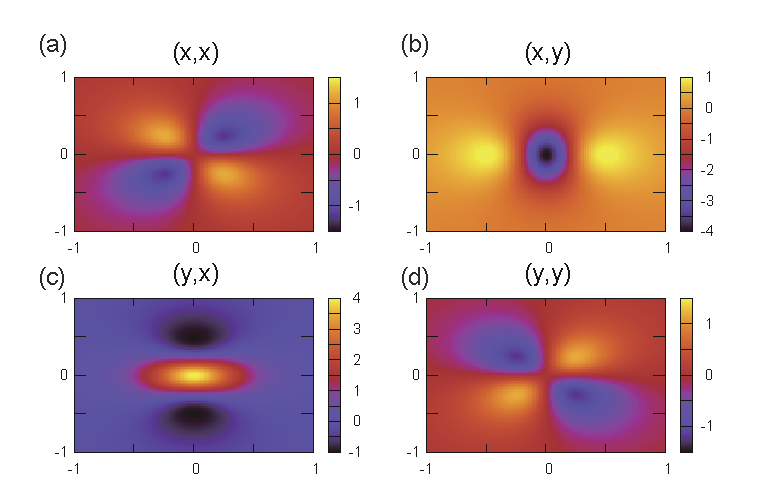
\includegraphics[width=\columnwidth]{fig_IFE/asym_density.pdf}
    \end{center}
    \caption{Values of $\varepsilon_{z\nu\delta}\partial_{\alpha}\partial_{\nu}g_{\delta\beta}$ around $(k_x,k_y)=(0,0)$ for the parameter $M/v=0.5$ with $(\alpha,\beta)=$ (a) $(x,x)$, (b) $(x,y)$, (c) $(y,x)$, and (d) $(y,y)$.}
    \label{fig:asym_density}
\end{figure}

Next, we investigate the dependence of the coefficient as a function of $M/v$ and estimate the magnitude of the IFE. As we can see in Eq.~\eqref{eq:quadrupole_density}, $a_{zxy}$ and $a_{zyx}$ are non-zero and others are zero for the current model. We define the symmetric part and anti-symmetric parts of $a_{\mu\alpha\beta}$ as $a_{\mu(\alpha\beta)}\coloneqq (a_{\mu\alpha\beta}+a_{\mu\beta\alpha})/2$ and $a_{\mu[\alpha\beta]}\coloneqq (a_{\mu\alpha\beta}-a_{\mu\beta\alpha})/2$, respectively. In Fig.~, we plot $a_{z(xy)}$ and $a_{z[xy]}$ as functions of the Fermi energy $\epsilon_\mathrm{F}$ at zero-temperature limit for several values of $M/v$. 


In this work, (conclusion)

We thank Teruaki Suyama, So Tanaka, and Ryutaro Tomomatsu for useful discussions and comments. HY is supported by Japan Society for the Promotion of Science (JSPS) KAKENHI Grant Number JP24KJ1109 and by MEXT Initiative to Establish Next-generation Novel Integrated Circuits Centers (X-NICS) Grant Number JPJ011438. TY is supported by Japan Society for the Promotion of Science (JSPS) KAKENHI Grant Numbers 25K07221 and JP30578216.

\bibliography{IFE.bib}

\end{document}